\section{Evaluations}\label{sec:evaluations}
\begin{figure}[t]
\centering
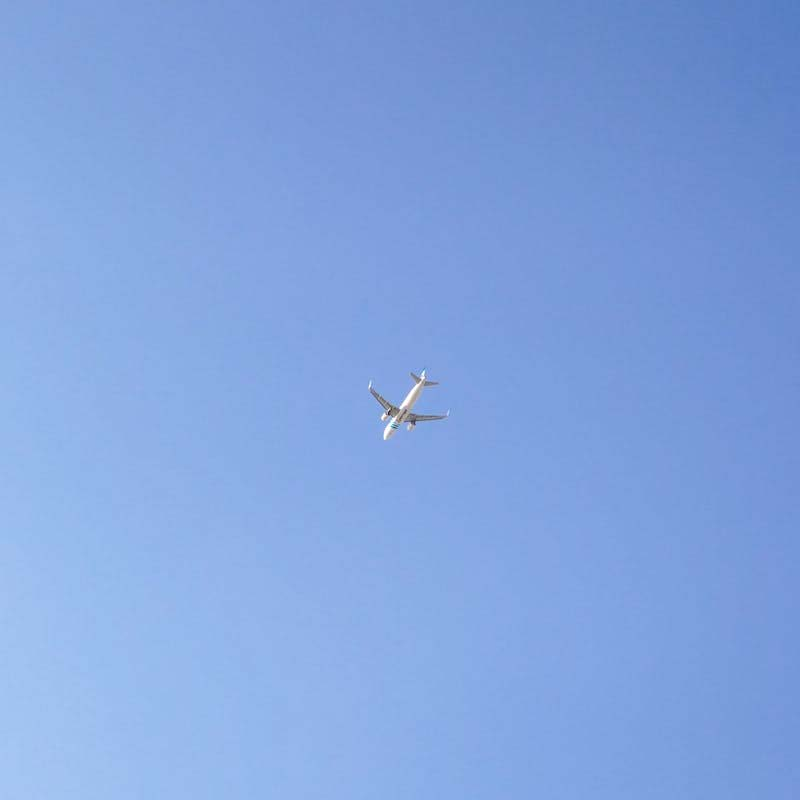
\includegraphics[width=0.2475\linewidth]{figures/airplane/6dof/input/0.jpg}\hfill
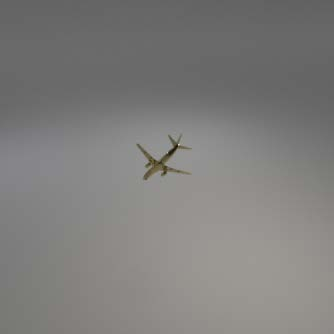
\includegraphics[width=0.2475\linewidth]{figures/airplane/6dof/output/0.jpg}\hfill
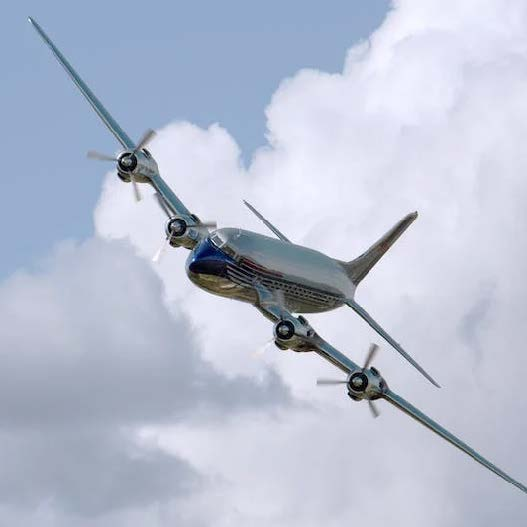
\includegraphics[width=0.2475\linewidth]{figures/airplane/6dof/input/1.jpg}\hfill
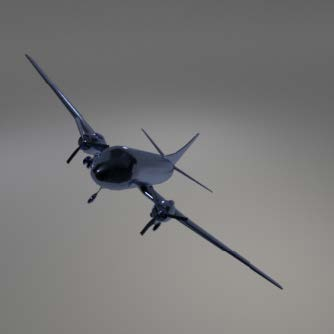
\includegraphics[width=0.2475\linewidth]{figures/airplane/6dof/output/1.jpg}
\caption{\textbf{OOD Single-Object 6-DoF Samples.} (\cref{sssec:single_6dof})
A sample 6-DoF reconstruction of real-world images.
The model is finetuned with only Blender renderings of toy airplanes that have a white backdrop.
See \cref{fig:single_6dof_samples_additional} for additional samples.
}
\label{fig:single_6dof_samples}
\end{figure}
To evaluate the ability of our proposed framework to generalize across distribution shifts, we design a number of focused evaluation settings.
We conduct experiments on synthetic data in order to quantitatively analyze model capability under controlled shifts.

\subsection{Compositional Generalization on CLEVR}\label{ssec:clevr}
An extension to CLEVR, known as CLEVR-CoGenT~\citep{johnson2017clevr}, serves as a benchmark for evaluating the \textit{compositional}-generalization capabilities of VQA models.
This benchmark assesses the model's ability to answer questions about scenes containing objects with unseen combinations of attributes.
During training, the dataset is structured such that particular types of objects are only assigned specific combinations of attributes (e.g.~blue cubes and red cylinders), while the testing data includes objects with attribute combinations not seen during training (e.g.~red cubes and blue cylinders).
We adapt this VQA dataset to our inverse-graphics problem domain, employing it for three primary purposes:
1) demonstrating that LLMs can effectively perform inverse graphics by testing on in-distribution (ID) data;
2) illustrating that LLMs exhibit robust compositional generalization to OOD data, while the baseline approach in NS-VQA~\citep{yi2018neural} struggles in this setting; and
3) exploring the data-efficiency of our framework.

\noindent\textbf{Setting.}
Following the setting of CLEVR-CoGenT, our training set consists of images of scenes containing objects with only a subset of possible attribute combinations (shape, size, material, and color).
In the ID condition, all cubes are rendered in gray, blue, brown, or yellow, and all cylinders are depicted in red, green, purple, or cyan.
In contrast, in the OOD condition the color palettes of the shapes are swapped.
Spheres are consistently depicted with all eight colors under both conditions.
We train both our proposed framework and NS-VQA, our neural-scene de-rendering baseline, on 4k images from the ID condition and evaluate them on 1k images from both the ID and OOD conditions. We follow CLEVR and randomly apply their set of synonyms on the categorical attributes.

\begin{table}[t]
\centering
\caption{
\textbf{CLEVR-CoGenT Results.} (\cref{ssec:clevr})
While both our proposed framework and the baseline, NS-VQA, and are able to achieve \textgreater 99\% accuracy on the ID condition, the baseline fails to generalize, with its shape-recognition accuracy dropping by 66.12\%.
\textit{Color}, \textit{Mat.}, and \textit{Shape} represent respective accuracies and $\uparrow$ indicates greater is better.
}
\begin{tabular}{lrrr|rrr}
\toprule
& \multicolumn{3}{c}{ID} & \multicolumn{3}{c}{OOD} \\
& Char & Float & NS-VQA & Char & Float & NS-VQA \\
\midrule
$\downarrow$L2 & 0.21 & 0.16 & 0.18 & 0.22 & 0.17 & 0.18 \\
$\uparrow$Size & 99.71 & 99.77 & 100.00 & 99.74 & 99.80 & 100.00 \\
$\uparrow$Color & 99.58 & 99.71 & 100.00 & 98.60 & 98.14 & 99.95 \\
$\uparrow$Shape & 99.51 & 99.59 & 100.00 & 93.50 & 93.14 & \fbox{33.88} \\
\bottomrule
\end{tabular}
\label{table:clevr}
\end{table}

\noindent\textbf{Evaluation Metrics.}
To evaluate attribute-recognition accuracy, we employ linear-sum assignment on pairwise Euclidean distances to match predicted and ground-truth objects.
However, since attribute-recognition accuracy does not account for missing or duplicated objects, we also evaluate the method's ability to produce accurate counts by computing the mean-absolute counting error between the predicted and ground-truth object sets across scenes (\textit{Count}).

\begin{wrapfigure}{R}{0.45\linewidth}
\centering
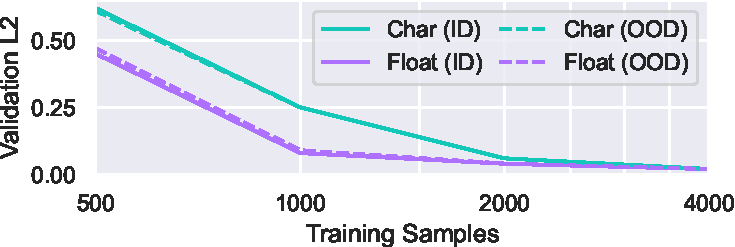
\includegraphics[width=\linewidth]{figures/clevr/data_efficiency_plot.pdf}
\caption{\textbf{CLEVR Data Efficiency.} (\cref{ssec:clevr})
Plot of the validation L2 positional error by the number of training samples.
We observe that the float-based model is consistently more data-efficient but that the difference between the models converges as the number of training samples reaches 4000.
See \cref{table:clevr_data_efficiency} for a full quantitative comparison.
}
\label{fig:clevr_data_efficiency}
\vspace{-0.5cm}
\end{wrapfigure}
\noindent\textbf{Results.}
Both our proposed framework and NS-VQA achieve \textgreater 99\% accuracy on the ID condition (\cref{table:clevr}), which underscores LLMs' ability to perform comparably with domain-specific modular designs.
However, when evaluated on the OOD condition, the shape-recognition accuracy of the baseline method drops substantially by 66.12\%, while the accuracy of our pipeline decreases by only 6.01\%.
Notably, when spheres, observed with all colors during training, are removed from the evaluation, the shape accuracy of NS-VQA plummets further to 0.03\%.
Illustrative reconstructions from the OOD condition can be seen in \cref{fig:clevr_samples}.

In terms of data efficiency, we find the float-based model to be much more efficient than the char-based model in estimating the positions of objects, but the difference diminishes as the number of samples reaches 4k (\cref{fig:clevr_data_efficiency}).
Hypothesizing that the char-based model has learned to compositionally retrieve the exact positions of (individual) objects from the training set rather than learning to effectively interpolate between training values, we measure 
the likelihood of predicting arbitrary three-decimal values.
Our findings reveal that the char-based model is 6.41 times more likely to predict a particular value if that discrete value was observed during training.
We further explore float-estimation dynamics in \cref{ssec:parameter_space_generalization}.

\subsection{Numeric Parameter-Space Generalization}\label{ssec:parameter_space_generalization}
In this section, we investigate the addition of a numeric head and the ability of our framework to generalize across parameter space.

\begin{figure*}[t]
\centering
\begin{subfigure}{.196\linewidth}
\centering
\raisebox{0cm}{
\includegraphics[width=\linewidth]{figures/2d/sparse_checkerboard.pdf}}
\caption{Train Distribution}\label{fig:2d_sparse_checkerboard}
\end{subfigure}
\hspace{-0.15cm}
\begin{subfigure}{.196\linewidth}
\centering
\raisebox{0cm}{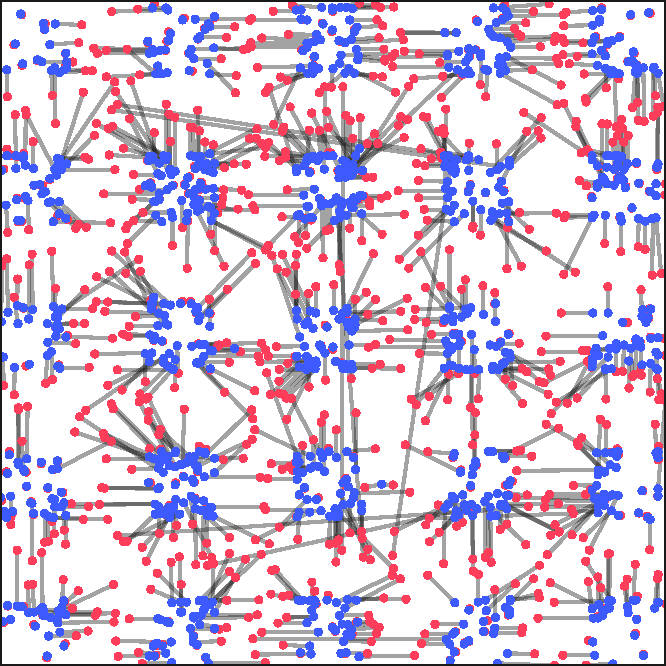
\includegraphics[width=\linewidth]{figures/2d/char_scatter.pdf}}
\caption{Char Model Pred.}\label{fig:2d_char_scatter}
\end{subfigure}
\hspace{-0.15cm}
\begin{subfigure}{.196\linewidth}
\centering
\raisebox{0cm}{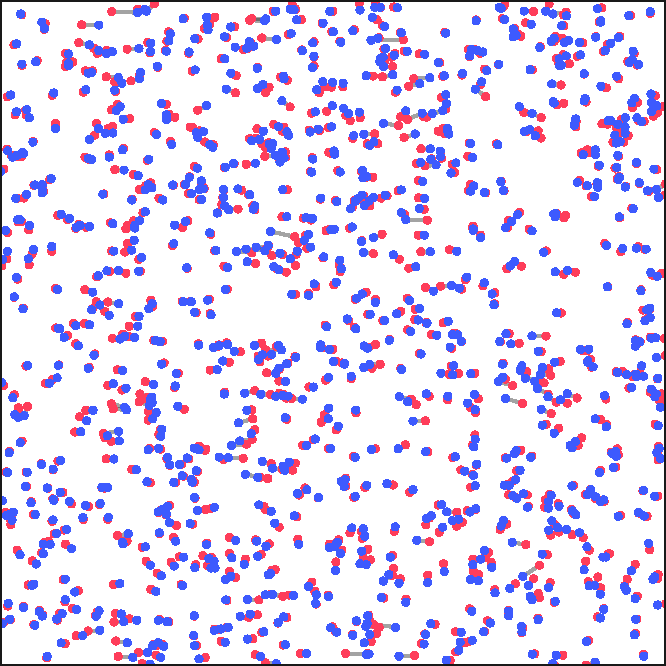
\includegraphics[width=\linewidth]{figures/2d/float_scatter.pdf}}
\caption{Float Model Pred.}\label{fig:2d_float_scatter}
\end{subfigure}
\begin{subfigure}{.196\linewidth}
\centering
\raisebox{0.0cm}{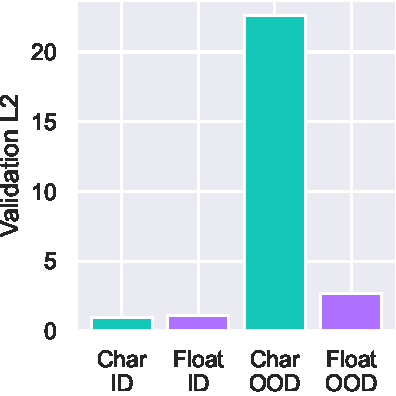
\includegraphics[width=\linewidth]{figures/2d/bar.pdf}}
\caption{ID--OOD}
\label{fig:2d_bar}
\end{subfigure}
\hfill
\begin{subfigure}{.196\linewidth}
\centering
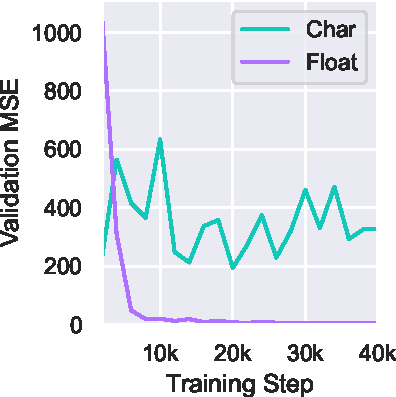
\includegraphics[width=\linewidth]{figures/2d/dynamics.pdf}
\caption{Dynamics}
\label{fig:2d_dynamics}
\end{subfigure}
\caption{\textbf{2D Parameter-Space Generalization.} (\cref{sssection:2d})
(a) Training positions are sampled from the checkerboard.
When evaluated on images with uniformly sampled positions, the char-based model fails to generalize outside the training distribution (b) while the float-based model effectively interpolates samples (c).
Randomly-sampled testing locations are shown in red and the corresponding predictions in blue.
(d) shows that while both methods well-estimate samples from the ID condition, the char-based model struggles to generalize.
(e) shows a plot of the model's validation MSE as a function of the number of training steps.
We observe that the training of the float-based model is much smoother and converges quickly.
}
\label{fig:2d}
\end{figure*}

\subsubsection{2D Parameter Space}\label{sssection:2d}
We begin by scrutinizing the framework's ability to generalize in 2D parameter space across range gaps.
To accomplish this, we create a dataset comprising 10k images, each featuring a red dot on a white background.
During training, the model is shown images where the location of the dot is sampled from a sparse checkerboard grid, as shown in \cref{fig:2d_sparse_checkerboard}.
During evaluation, the model is shown 1k images where the dot's location is uniformly sampled across the square; points lying outside the checkerboard are effectively OOD inputs. 

\noindent\textbf{Results.}
As shown in \cref{fig:2d_char_scatter}, the char-based model exhibits significant overfitting to the training distribution, consistently predicting dot locations restricted to the checkerboard distribution observed during training.
In contrast, the float-based model is able to effectively generalize across parameter space, adapting to the uniformly sampled testing distribution during evaluation (\cref{fig:2d_float_scatter}).
Although the float-based model exhibits a slight positional bias toward predicting positions on the grid (as evidenced by the higher OOD error),  
the disparity in the ID--OOD validation-L2 performance gap of the char-based model is 14 times as high as that of the float-based model (\cref{fig:2d_bar}).
Moreover, the validation MSE of the float-based model converges quickly to near zero, while the error of the char-based model is much less stable over time (\cref{fig:2d_dynamics}), suggesting that the float-based model learns smooth, low-dimensional representations of the space while the char-based variant may not.

\subsubsection{SO(3) Parameter Space}\label{sssec:so3}
\begin{figure}
\centering
\fbox{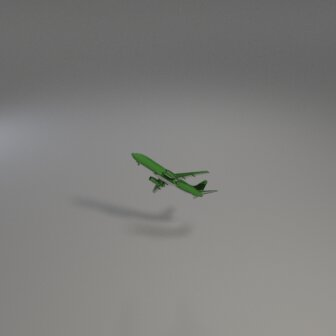
\includegraphics[width=0.4\linewidth]{figures/samples/so3.jpg}}
\begin{minted}[breaklines]{python}
add(shape='airliner', size='tiny', color='green', material='matte', rotation=(-0.798, 0.124, 0.590, -0.562, -0.507, -0.654))
\end{minted}
\caption{\textbf{SO(3) Range-Gap Train Sample.} (\cref{sssec:so3})}
\label{fig:code_so3}
\end{figure}
We continue our parameter-space evaluation within the more complex task of SO(3)-pose estimation of orientable objects.
For this, we make use of five toy-airplane assets sourced from Super-CLEVR~\citep{Li_2023_CVPR}. 
We construct a training dataset of 10k images of single planes at a fixed location and sampled attributes identical to those in CLEVR.
Extending the range-gap setup used in \cref{sssection:2d}, the airplanes are assigned random extrinsic-Euler rotations, where the components are sampled from ranges containing inserted gaps (e.g., $[-\frac{\pi}{20},\frac{\pi}{20}]$).
A visual depiction of this space is provided in \cref{fig:so3_range}, with the training values exclusively sampled from the blue ranges.
During testing, we invert the gaps to assess OOD generalization.
We evaluate performance across intrinsic-Euler, extrinsic-Euler, axis-angle, and 6D~\citep{Zhou_2019_CVPR} representations.

\noindent\textbf{Results.}
We report full results in \cref{table:so3} and here discuss only results from the best-performing representation variants in each evaluation, being intrinsic-Euler for char and 6D for float in ID, and axis-angle for both in OOD.
We do so to avoid biasing results with a representation that is better suited for one model variant or the other.

As depicted in \cref{fig:so3_bar}, the error of the char-based model is 2.64 times higher than that of the float-based model when evaluated in-distribution.
Upon testing in the OOD condition, the disparity is nearly consistent at 2.52 times that observed in the ID scenario, with the ID--OOD gap of the char-based model being 2.21 times that observed in the float-based variant.
We attribute the superiority of the float-based model across both conditions to the increased data dimensionality.
Additionally, the lesser performance decline observed when evaluating on the OOD training gaps further underscores the parameter-space efficiency of the float-based model.

\subsection{6-DoF Pose Estimation}\label{ssec:6dof}
\begin{figure}[t]
\centering
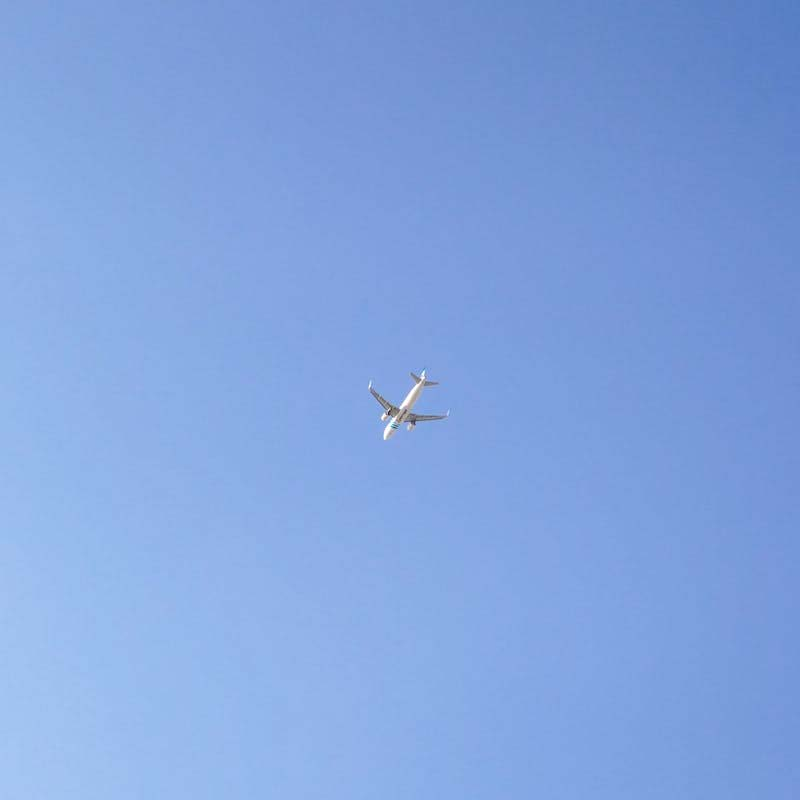
\includegraphics[width=0.2475\linewidth]{figures/airplane/6dof/input/0.jpg}\hfill
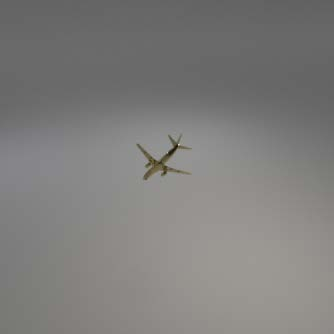
\includegraphics[width=0.2475\linewidth]{figures/airplane/6dof/output/0.jpg}\hfill
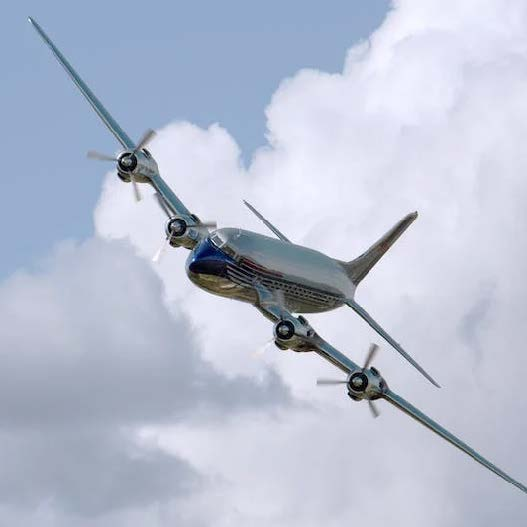
\includegraphics[width=0.2475\linewidth]{figures/airplane/6dof/input/1.jpg}\hfill
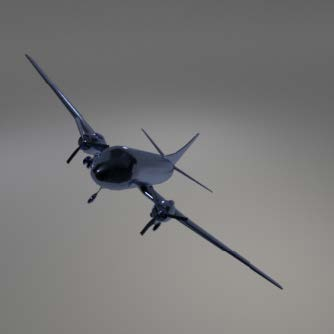
\includegraphics[width=0.2475\linewidth]{figures/airplane/6dof/output/1.jpg}
\caption{\textbf{OOD Single-Object 6-DoF Samples.} (\cref{sssec:single_6dof})
A sample 6-DoF reconstruction of real-world images.
The model is finetuned with only Blender renderings of toy airplanes that have a white backdrop.
See \cref{fig:single_6dof_samples_additional} for additional samples.
}
\label{fig:single_6dof_samples}
\end{figure}
We examine the ability of our framework to scale in tackling a more challenging inverse-graphics task: that of 6-DoF-pose estimation.
Our exploration begins with an evaluation on single-object images, encompassing both quantitative and qualitative assessments, where we illustrate the framework's ability to generalize across visual domain shifts.
We subsequently extend the setting to include more-complex (albeit, synthetic) multi-object scenes, demonstrating promising results for scene estimation, handling larger collections (\textgreater 100) of diverse assets. 
\begin{table}[t]
\centering
\caption{
\textbf{CLEVR-CoGenT Results.} (\cref{ssec:clevr})
While both our proposed framework and the baseline, NS-VQA, and are able to achieve \textgreater 99\% accuracy on the ID condition, the baseline fails to generalize, with its shape-recognition accuracy dropping by 66.12\%.
\textit{Color}, \textit{Mat.}, and \textit{Shape} represent respective accuracies and $\uparrow$ indicates greater is better.
}
\begin{tabular}{lrrr|rrr}
\toprule
& \multicolumn{3}{c}{ID} & \multicolumn{3}{c}{OOD} \\
& Char & Float & NS-VQA & Char & Float & NS-VQA \\
\midrule
$\downarrow$L2 & 0.21 & 0.16 & 0.18 & 0.22 & 0.17 & 0.18 \\
$\uparrow$Size & 99.71 & 99.77 & 100.00 & 99.74 & 99.80 & 100.00 \\
$\uparrow$Color & 99.58 & 99.71 & 100.00 & 98.60 & 98.14 & 99.95 \\
$\uparrow$Shape & 99.51 & 99.59 & 100.00 & 93.50 & 93.14 & \fbox{33.88} \\
\bottomrule
\end{tabular}
\label{table:clevr}
\end{table}
\subsubsection{Single-Object 6-DoF}\label{sssec:single_6dof}
We first evaluate our framework's ability to scale to single-object 6-DoF pose estimation. The float- and char-based models are assessed quantitatively using rendered images. 

\noindent\textbf{Setting.}
We extend the setting used in \cref{sssec:so3} but unfreeze the previously fixed 3D position and assign it a randomly sampled value.
We expand the number of colors used in the dataset to 133\footnote{\url{https://simple.wikipedia.org/wiki/List_of_Crayola_crayon_colors}} to better emulate the diversity observed in the real world.
Differing from the previous setup, we fix the size of the objects due to the relative depth--scale ambiguity of the toy airplanes.
To evaluate our framework's ability to scale beyond data-constrained scenarios, we render a training dataset of one-million images.
Following the rotation-representation results of \cref{sssec:so3}, we use the intrinsic-Euler representation for the char-based model and the 6D representation for the float-based model as their use led to the greatest ID performance.

\noindent\textbf{Results.}
\cref{table:single_6dof} illustrates that, under this non-data-constrained scenario, both model variants effectively capture the dynamics of the task
The models both notably exhibit an order of magnitude lower positional error than in the CLEVR setting, despite the addition of 3D orientation and an additional positional dimension, and achieve rotational error 28\% of that observed in the ID portion of the SO(3) range-gap evaluation.
This reinforces the earlier observation from the CLEVR data-efficiency evaluation that, given sufficient data, the model variants exhibit a similar performance ceiling.
Still, neither achieves the level of precision necessary to be directly constrained by the three-decimal-place discretization applied to numeric quantities throughout the evaluations nor the 16-bit training precision in the case of the float-based model.
See \cref{sec:further_training_details} for further training details.

As part of our evaluation, we also qualitatively examine the ability of the model to transfer from the renders of toy planes with a solid-white background, on which it was fine-tuned, to estimating the pose and attributes of planes in real-world images.
We provide qualitative samples of our model's generalization to such images in \cref{fig:single_6dof_samples}.
We observe encouraging generalization across the majority of images tested, despite the lack of augmentation or domain-specific inductive bias applied during the training process.
However, it is difficult to quantitatively evaluate such model performance due to a lack of paired real-world data in line with our compositional task.
As a proxy for such an evaluation, we introduce a synthetic setting in \cref{sssec:scene_6dof} to quantitatively evaluate the ability of our framework to generalize across visual domains.

\subsubsection{Scene-Level 6-DoF}\label{sssec:scene_6dof}
\begin{table}[t]
\centering
\caption{
\textbf{CLEVR-CoGenT Results.} (\cref{ssec:clevr})
While both our proposed framework and the baseline, NS-VQA, and are able to achieve \textgreater 99\% accuracy on the ID condition, the baseline fails to generalize, with its shape-recognition accuracy dropping by 66.12\%.
\textit{Color}, \textit{Mat.}, and \textit{Shape} represent respective accuracies and $\uparrow$ indicates greater is better.
}
\begin{tabular}{lrrr|rrr}
\toprule
& \multicolumn{3}{c}{ID} & \multicolumn{3}{c}{OOD} \\
& Char & Float & NS-VQA & Char & Float & NS-VQA \\
\midrule
$\downarrow$L2 & 0.21 & 0.16 & 0.18 & 0.22 & 0.17 & 0.18 \\
$\uparrow$Size & 99.71 & 99.77 & 100.00 & 99.74 & 99.80 & 100.00 \\
$\uparrow$Color & 99.58 & 99.71 & 100.00 & 98.60 & 98.14 & 99.95 \\
$\uparrow$Shape & 99.51 & 99.59 & 100.00 & 93.50 & 93.14 & \fbox{33.88} \\
\bottomrule
\end{tabular}
\label{table:clevr}
\end{table}
\begin{figure}[t]
\centering
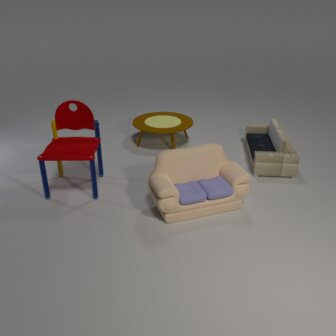
\includegraphics[width=0.2475\linewidth]{figures/shapenet/OOD/0_in.jpg}\hfill
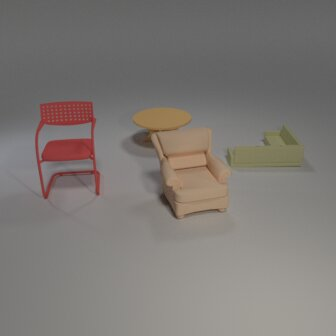
\includegraphics[width=0.2475\linewidth]{figures/shapenet/OOD/0_out.jpg}\hfill
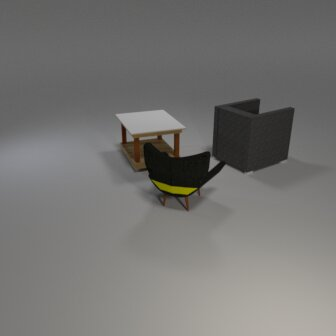
\includegraphics[width=0.2475\linewidth]{figures/shapenet/OOD/1_in.jpg}\hfill
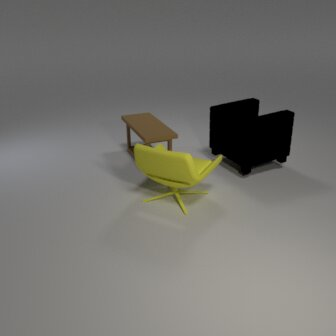
\includegraphics[width=0.2475\linewidth]{figures/shapenet/OOD/1_out.jpg}
\caption{\textbf{OOD ShapeNet 6-DoF Samples.} (\cref{sssec:scene_6dof})
Two sample reconstructions from the OOD ShapeNet 6-Dof pose-estimation experiment.
Left to right: input, output.
We evaluate on assets not shown during training, with out-of-distribution textures.
See \Cref{fig:scene_6dof_ood_samples_additional} for additional samples.
}
\label{fig:scene_6dof_ood_samples}
\end{figure}
In this section, we explore the scalability of our framework to scene-level 6-DoF-pose estimation, featuring 3-5 objects per scene and a much-expanded array of assets.
This experiment not only assesses performance under more-challenging conditions, but also enables a quantitative evaluation on the framework's ability to generalize to scenes with OOD visual appearance.

\noindent\textbf{Setting.}
We construct an expanded CLEVR-like image--scene dataset, incorporating objects sourced from ShapeNet~\citep{shapenet2015}.
The dataset comprises 56 chair types, 35 sofa types, and 47 table types.
We remove the size and material attributes used in CLEVR, but employ the expanded color set used in \cref{sssec:single_6dof} to randomly color the objects.
After doing so, the total number of possible combinations of attributes is 191-fold that used in the CLEVR-CoGenT experiment.
Differing from previous evaluations, we also vary the pitch of the camera and the radius of its arc, but maintain a fixed camera focal point.
Returning from the million-image single-object 6-DoF evaluation to a relatively data-constrained setting, we render 10k training images and evaluate the framework on three conditions, each with 1K images:
(1) ID, which matches the training distribution of scenes with solid-colored objects;
(2) OOD texture (OOD-T), where the same object assets are used as in ID but the objects are rendered with original ShapeNet textures instead of the randomly assigned solid colors;
and (3) OOD encompassing both unseen objects and original ShapeNet textures (OOD-T+S). We use this to emulate the distribution shift of modeling real-world scenes, while facilitating quantitative evaluation.

\noindent\textbf{Results.}
We observe that both approaches scale to the task, though the float-based model outperforms -- or ties with -- the char-based variant across evaluations (\cref{table:scene_6dof}).
This disparity is emphasized in the OOD-T+S setting where scene-level chamfer distance of the char-based model jumps from being approximately twice that of the float-based variant in the ID and OOD-T evaluations to being 5.67 times as much.

There is a decrease in performance observed when stepping to the OOD-T setting, which is most-strongly observed in the count error (x8 for both) and the shape-recognition accuracy (-20.49\% in char and -15.05\% in float).
We empirically attribute this to the model occasionally explaining some multi-color textured objects using a composition of multiple, solid-color assets.
Quantitatively supporting this, the performance decrease is not as strongly reflected in scene-level chamfer distance (x2.6 for both).

See \cref{fig:scene_6dof_ood_samples} for samples reconstructions from OOD-T+S and \cref{fig:scene_6dof_id_samples_additional} for samples from the ID setting.
We additionally test our model on real-world samples, but find that it fails to consistently generalize (\cref{fig:scene_6dof_rw_samples}).
We attribute this failure partially to limitations in the camera-position training distribution.